% handout
\documentclass[11pt,final,usepdftitle=false]{beamer}
\mode<presentation>
\usetheme{ln12en}
\graphicspath{{\logopath}{\picspath}{\figspath}{./logos/}{./pics/}{./figs/}}
\usepackage{listings}
%\usepackage{bera}
\usepackage{inconsolata}
\usepackage{moresize}
\usepackage{ucs}
\usepackage{framed}
\usepackage{adjustbox}
%\renewcommand*\ttdefault{cmvtt}


\hypersetup{pdftitle={Lucas Nussbaum - systemd}}
\title{systemd}
\authorteaching
\instituteiutlp
\newcommand{\tilda}{\textasciitilde{}}
\date{}


\AtBeginSection[]
{
  \begin{frame}
    \frametitle{Plan}
    \tableofcontents[currentsection]
  \end{frame}
}

\usepackage{tikz}
\usetikzlibrary{shapes,arrows,positioning}
\newcommand{\Gentsroom}{{\fontfamily{mvs}\fontencoding{U}\fontseries{m}\fontshape{n}\selectfont\char120}}

\begin{document}

\frame{\titlepage}

\begin{frame}{Init system}
\begin{itemize}
\item First process started by the kernel (pid 1)
	\hbr
\item Responsible for bringing up the rest of userspace
	\begin{itemize}
		\item Mounting filesystems
		\item Starting services
		\item \ldots
	\end{itemize}
	\hbr
\item Also the parent for orphan processes
	\hbr
\item Traditional init system on Linux: sysVinit
	\begin{itemize}
		\item Inherited from Unix System V
		\item With additional tools (insserv, startpar) to handle dependencies and parallel initialization
	\end{itemize}
\end{itemize}
\end{frame}

\begin{frame}{systemd}
	\begin{itemize}
		\item Written (since 2010) by Lennart Poettering (Red Hat) and others
			\hbr
		\item Now the default on most Linux distributions
			\hbr
		\item Shifts the scope from \textsl{starting all services} (sysVinit) to\\
			\alert{managing the system and all services}
			\hbr
		\item Key features:
			\begin{itemize}
				\item Relies on cgroups for
					\begin{itemize}
						\item Services supervision
						\item Control of services execution environment
					\end{itemize}
					\hbr
				\item Declarative syntax for unit files $\leadsto$ more efficient/robust
					\hbr
				\item Socket activation (on-demand startup of services)
					\hbr
				\item Nicer user interface (systemctl \& friends)
			\end{itemize}
			\hbr
		\item Additional features: logging, timer units (cron-like), user sessions handling, containers management
	\end{itemize}
\end{frame}

\begin{frame}{Behind the scenes: cgroups}
\begin{itemize}
\item Abbreviated from \textsl{control groups}
\hbr
\item Linux kernel feature
\hbr
\item Limit, account for and isolate \alert{processes and their resource usage} (CPU, memory, disk I/O, network, etc.)
\hbr
\item Related to \textsl{namespace isolation}:
	\begin{itemize}
		\item Isolate processes from the rest of the system
			\hbr
		\item \textsl{Chroots on steroids}
			\hbr
		\item PID, network, UTS, mount, user, etc.
	\end{itemize}
			\hbr
		\item LXC, Docker $\approx$ cgroups + namespaces (+ management tools)
\end{itemize}
\end{frame}

\begin{frame}{cgroups and systemd}
	\begin{itemize}
	\item Each service runs in its own cgroup
		\hhbr
	\item Enables:
		\begin{itemize}
			\item Tracking and killing all processes created by each service
				\hhbr
			\item Per-service accounting and resources allocation/limitation
		\end{itemize}
		\hhbr
	\item Previously, with sysVinit:
		\begin{itemize}
			\item No tracking of which service started which processes
				\begin{itemize}
					\item PID files, or hacks in init scripts: \texttt{pidof} / \texttt{killall} / \texttt{pgrep}
						\hhbr
					\item Hard to completely terminate a service (left-over CGI scripts when killing Apache)
				\end{itemize}
				\hbr
			\item No resources limitation (or using \texttt{setrlimit} (= \texttt{ulimit}), which is per-process, not per-service)
		\end{itemize}
	\hhbr
	\item Also isolate user sessions $\leadsto$ kill all user processes (not by default)
	\hhbr
\item More information: \href{http://0pointer.net/blog/projects/cgroups-vs-cgroups.html}{\ul{Control Groups vs. Control Groups}} and\\ \href{http://0pointer.net/blog/projects/systemd-for-admins-2.html}{\ul{Which Service Owns Which Processes?}}
\end{itemize}
\end{frame}



\begin{frame}{\texttt{systemd-cgls}: visualizing cgroup hierarchy}
% export GTK_MODULES=/usr/lib/gtk-3.0/modules/libgtk-vector-screenshot.so
% take-vector-screenshot
\hbr

\includegraphics[height=0.9\textheight]{figs/systemd-cgls}
\end{frame}

\begin{frame}{\texttt{systemd-cgtop}: per-service resources usage}
\begin{framed}

\includegraphics[width=1\textwidth]{figs/systemd-cgtop}
\end{framed}
Note: requires enabling \texttt{CPUAccounting}, \texttt{BlockIOAccounting}, \texttt{MemoryAccounting}
\end{frame}

\begin{frame}{Managing services with \texttt{systemctl}}
	\begin{itemize}
		\item What is being manipulated is called a  \textsl{unit}: services (.service), mount points (.mount), devices (.device), sockets (.socket), etc.
			\hbr
		\item Basic commands:
\hbr
	\end{itemize}
	\resizebox{\textwidth}{!}{
	\begin{tabular}{|c|c|c|}
		\hline
		sysVinit & systemd & notes \\
		\hline
		service foo start & systemctl start foo & \\
		service foo stop & systemctl stop foo & \\
		service foo restart & systemctl restart foo & \\
		service foo reload & systemctl reload foo & \\
		service foo condrestart & systemctl condrestart foo & restart if already running \\
		update-rc.d foo enable & systemctl enable foo & auto-start at next boot \\
		update-rc.d foo disable & systemctl disable foo & disable auto-start \\
		& systemctl is-enabled foo & \\
		\hline
	\end{tabular}}
	\begin{itemize}
		\item There's auto-completion (\texttt{apache2} and \texttt{apache2.service} work)
		\hbr
		\item Several services can be specified:\\
			\texttt{systemctl restart apache2 postgresql}
		\hbr
	\end{itemize}
\end{frame}

\begin{frame}{systemd and runlevels}
	\begin{itemize}
		\item With sysVinit, runlevels control which services are started automatically
			\begin{itemize}
				\item 0 = halt; 1 = single-user / minimal mode; 6 = reboot
				\item Debian: no difference between levels 2, 3, 4, 5 (multi-user)
				\item RHEL: 3 = multi-user text, 5 = multi-user graphical
			\end{itemize}
			\hbr
		\item systemd replaces runlevels with \alert{targets}:
			\begin{itemize}
				\item Configured using symlinks farm in \texttt{/etc/systemd/system/\textbf{target}.wants/}
					\hbr
				\item \texttt{systemctl enable}/\texttt{disable} manipule those symlinks
					\hbr
				\item \texttt{systemctl mask} disables the service and prevents it from being started manually
					\hbr
				\item The default target can be configured with\\ \texttt{systemctl get-default/set-default}
					\hbr
				\item More information: \href{http://0pointer.net/blog/projects/three-levels-of-off.html}{\ul{The Three Levels of "Off"}}
			\end{itemize}
	\end{itemize}
\end{frame}

\begin{frame}[fragile]{Default targets (\texttt{bootup(7)})}
\begin{center}
\begin{adjustbox}{height=0.45\textheight,keepaspectratio}
\begin{lstlisting}[basicstyle=\ttfamily\tiny,escapeinside={<<}]
local-fs-pre.target
         |
         v
(various mounts and   (various swap   (various cryptsetup
 fsck services...)     devices...)        devices...)       (various low-level   (various low-level
         |                  |                  |             services: udevd,     API VFS mounts:
         v                  v                  v             tmpfiles, random     mqueue, configfs,
  local-fs.target      swap.target     cryptsetup.target    seed, sysctl, ...)      debugfs, ...)
         |                  |                  |                    |                    |
         \__________________|_________________ | ___________________|____________________/
                                              \|/
                                               v
                                        sysinit.target
                                               |
          ____________________________________/|\________________________________________
         /                  |                  |                    |                    \
         |                  |                  |                    |                    |
         v                  v                  |                    v                    v
     (various           (various               |                (various          rescue.service
    timers...)          paths...)              |               sockets...)               |
         |                  |                  |                    |                    v
         v                  v                  |                    v               <\textbf{rescue.target}<
   timers.target      paths.target             |             sockets.target
         |                  |                  |                    |
         \__________________|_________________ | ___________________/
                                              \|/
                                               v
                                         basic.target
                                               |
          ____________________________________/|                                 emergency.service
         /                  |                  |                                         |
         |                  |                  |                                         v
         v                  v                  v                                  <\textbf{emergency.target}<
     display-        (various system    (various system
 manager.service         services           services)
         |             required for            |
         |            graphical UIs)           v
         |                  |            <\textbf{multi-user.target}<
         |                  |                  |
         \_________________ | _________________/
                           \|/
                            v
                      <\textbf{graphical.target}<
\end{lstlisting}
\end{adjustbox}
\end{center}
\end{frame}

\begin{frame}{Exploring the system status}
\begin{itemize}
\item Listing units with \texttt{systemctl list-units} (or just \texttt{systemctl}):
\begin{itemize}
\item active units: \texttt{systemctl}
\hhbr
\item List only services: \texttt{systemctl -t service}
\hhbr
\item List units in failed state: \texttt{systemctl --failed}
\end{itemize}
\hbr
\item Whole system overview: \texttt{systemctl status}
\end{itemize}
\end{frame}

\begin{frame}{\texttt{systemctl status \textsl{\tt service}}}
\br
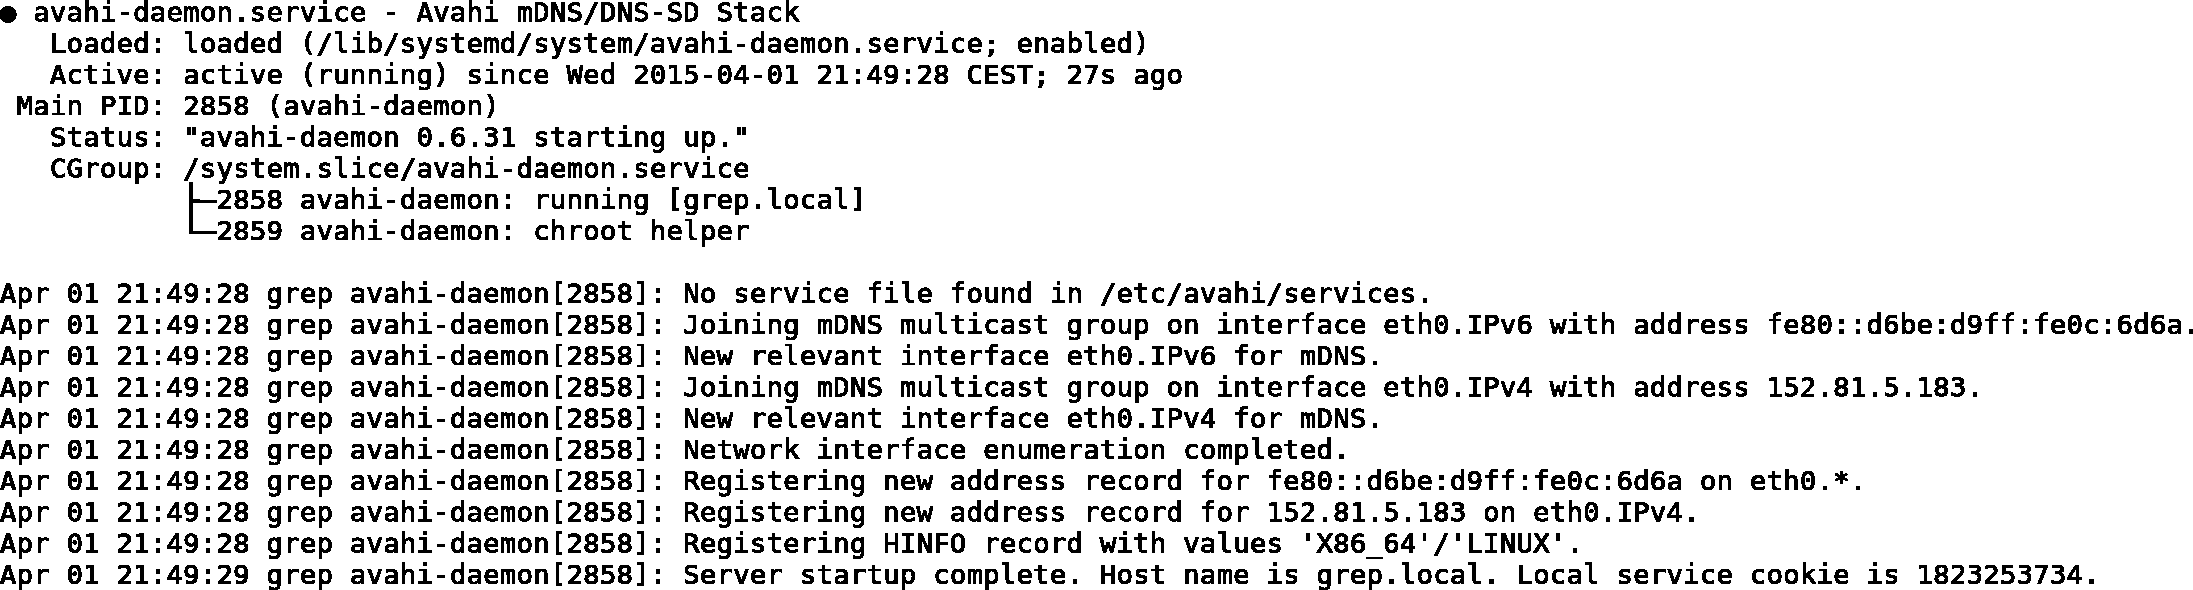
\includegraphics[width=1.5\textwidth]{figs/systemctl-status}
\hbr
Includes:
\begin{itemize}
\item Service name and description, state, PID
\item Free-form status line from \texttt{systemd-notify(1)} or \texttt{sd\_notify(3)}
\item Processes tree inside the cgroup
\item Last lines from journald (syslog messages and stdout/stderr)
\end{itemize}
\end{frame}

\begin{frame}{Writing unit files}
\begin{itemize}
\item With sysVinit: shell scripts in \texttt{/etc/init.d/}
\begin{itemize}
\item Long and difficult to write
\item Redundant code between services
\item Slow (numerous forks() calls)
\end{itemize}
\hbr
\item With systemd: declarative syntax (.desktop-like)
\begin{itemize}
\item Most of the intelligence is moved from the script to systemd
\item Covers most of the needs -- shell scripts can still be used if needed
\item Can use includes and overrides
\item View a unit file for a known service: \texttt{systemctl cat atd.service}
\item Or just find the file under \texttt{/lib/systemd/system/} (system defaults) or \texttt{/etc/systemd/system} (local overrides)
\end{itemize}
\end{itemize}
\end{frame}

\begin{frame}[fragile]{Simple example: atd}
\begin{lstlisting}[basicstyle=\ttfamily\normalsize,escapeinside={||}]
[Unit]
Description=Deferred execution scheduler
|\alert{\# Pointer to documentation shown in systemctl status}|
Documentation=man:atd(8)

[Service]
|\alert{\# Command to start the service}|
ExecStart=/usr/sbin/atd -f
IgnoreSIGPIPE=false |\alert{\# Default is true}|

[Install]
|\alert{\# Indicates reverse-dependency}|
WantedBy=multi-user.target
\end{lstlisting}
\end{frame}

\begin{frame}[fragile]{Common options}
\hbr
\begin{itemize}
\item Documented in \texttt{systemd.unit(5)} ([Unit]), \texttt{systemd.service(5)} ([Service]), \texttt{systemd.exec(5)} (execution environment)
\hbr
\item Show all options for a given service:\\
\texttt{systemctl show atd}
\hbr
	\item Sourcing a configuration file:\\
\texttt{EnvironmentFile=-/etc/default/ssh}\\
\texttt{ExecStart=/usr/sbin/sshd -D \$SSHD\_OPTS}
\hbr
\item Using the \texttt{\$MAINPID} magic variable:\\
\texttt{ExecReload=/bin/kill -HUP \$MAINPID}
\hbr
\item Auto-restart a service when crashed:\\
\texttt{Restart=on-failure}
\hbr
\item Conditional start:\\
\texttt{ConditionPathExists=!/etc/ssh/sshd\_not\_to\_be\_run}\\
Also conditions on architecture, virtualization, kernel command-line, AC power, path properties, etc.
\end{itemize}
\end{frame}

\begin{frame}{Options for isolation and security}
	\begin{itemize}
		\item Use a network namespace to isolate the service from the network:\\
			\texttt{PrivateNetwork=yes}
			\hbr
		\item Use a filesystem namespaces:
			\begin{itemize}
				\item To provide a service-specific \texttt{/tmp} directory:\\
					\texttt{PrivateTmp=yes}
					\hbr
				\item To make some directories inaccessible or read-only:\\
					\texttt{InaccessibleDirectories=/home}\\
					\texttt{ReadOnlyDirectories=/var}
			\end{itemize}
			\hbr
		\item Specify the list of \texttt{capabilities(7)} for a service:\\
			\texttt{CapabilityBoundingSet=CAP\_CHOWN CAP\_KILL}\\
			Or just remove one:\\
			\texttt{CapabilityBoundingSet=~CAP\_SYS\_PTRACE}
			\hbr
		\item Disallow forking:\\
			\texttt{LimitNPROC=1}
	\end{itemize}
\end{frame}
\begin{frame}{Options for isolation and security (2)}
\begin{itemize}
		\item Run as user/group: \texttt{User=}, \texttt{Group=}
			\hbr
		\item Run service inside a chroot:\\
			\texttt{RootDirectory=/srv/chroot/foobar}\\
			\texttt{ExecStartPre=/usr/local/bin/setup-foobar-chroot.sh}\\
			\texttt{ExecStart=/usr/bin/foobard}\\
			\texttt{RootDirectoryStartOnly=yes}
			\hbr
		\item Control CPU shares, memory limits, block I/O, swapiness:\\
			\texttt{CPUShares=1500}\\
			\texttt{MemoryLimit=1G}\\
			\texttt{BlockIOWeight=500}\\
			\texttt{BlockIOReadBandwith=/var/log 5M}\\
			\texttt{ControlGroupAttribute=memory.swappiness 70}
			\hbr
		\item More information:
				\href{http://0pointer.net/blog/projects/security.html}{\ul{Securing your services}},
				\href{http://0pointer.net/blog/projects/changing-roots.html}{\ul{Changing roots}},
				\href{http://0pointer.net/blog/projects/resources.html}{\ul{Managing resources}}
	\end{itemize}
\end{frame}

\end{document}
